\documentclass[10.5pt,a4paper]{article}

% --------------------------------------------------
% Packages
% --------------------------------------------------
\usepackage[margin=0.72in]{geometry}
\usepackage{amsmath}
\usepackage{booktabs}
\usepackage{graphicx}
\usepackage{float}
\usepackage{array}
\usepackage{enumitem}
\usepackage{xcolor}
\usepackage{hyperref}
\usepackage{caption}
\usepackage{subcaption}

\hypersetup{
    colorlinks=true,
    linkcolor=black,
    urlcolor=blue,
    citecolor=black
}

\setlength{\parindent}{0pt}
\setlength{\parskip}{3pt}

\setlist[itemize]{nosep,leftmargin=*}
\setlist[enumerate]{nosep,leftmargin=*}

\captionsetup{
    font=small,
    labelfont=bf
}

% --------------------------------------------------
% Title
% --------------------------------------------------
\title{
    \vspace{-1cm}
    \textbf{Polynomial Regression}\\
    \large Machine Learning Assignment
}

\author{
    \textbf{Yashwanth}\\
    Roll Number: BT2024103\\
    GitHub Repository:
    \href{https://github.com/BT2024103/polynomial_regression/}
    {\texttt{github.com/BT2024103/polynomial\_regression}}
}

\date{}

% --------------------------------------------------
% Document
% --------------------------------------------------
\begin{document}

\maketitle

% ==================================================
\section{Introduction}
% ==================================================

This assignment focuses on predicting a continuous target variable $y$
using polynomial regression on two personalized datasets, \texttt{var1}
and \texttt{var2}. Each dataset contains different numbers of input
variables and has a different maximum permitted polynomial degree.

For \texttt{var1}, six input variables $(x_1,\ldots,x_6)$ are provided,
with a maximum polynomial degree of 10. For \texttt{var2}, three input
variables $(x_1,x_2,x_3)$ are provided, with a maximum polynomial degree
of 20.

The objective is to select an appropriate polynomial degree using
cross-validation, train the final model on the complete training data,
and generate predictions for the provided test datasets.

The primary evaluation metrics are Mean Squared Error (MSE) and the
coefficient of determination ($R^2$).

% ==================================================
\section{Methodology}
% ==================================================

The same general workflow is followed for both problems:

\begin{enumerate}
    \item Load the training dataset and separate input variables $X$
    from the target $y$.
    \item Generate polynomial features up to the candidate degree.
    \item Evaluate polynomial degrees 1 through the maximum using
    5-fold cross-validation with Ridge regression.
    \item Select the degree that minimises the mean validation MSE.
    \item Retrain using \texttt{RidgeCV} over a fine logarithmic grid
    of regularization parameters on the complete training set.
    \item Apply the trained pipeline to the test dataset to generate
    predictions.
    \item Save the required prediction CSV file.
\end{enumerate}

Polynomial features are generated as total-degree expansions.
For three variables and degree two, the feature expansion contains

\[
1,\ x_1,\ x_2,\ x_3,\ x_1^2,\ x_1x_2,\ x_1x_3,\
x_2^2,\ x_2x_3,\ x_3^2.
\]

A degree-$d$ expansion includes all monomials for which the sum of
exponents is at most $d$.

All features are standardized prior to regression.  Ridge
regularization is used throughout to control the effect of the large
number of polynomial features, especially at higher degrees.  The
regularization parameter $\alpha$ is selected automatically by
\texttt{RidgeCV} using cross-validation.

The implementation uses a \texttt{scikit-learn} \texttt{Pipeline}
combining \texttt{PolynomialFeatures}, \texttt{StandardScaler}, and
\texttt{RidgeCV}, with \texttt{n\_jobs=-1} for parallel cross-validation.

% ==================================================
\section{Problem 1: \texttt{var1}}
% ==================================================

\subsection{Dataset}

The \texttt{var1} dataset is associated with the problem of
\emph{Power Plant Steam Turbine Optimization}. It contains six input
variables,

\[
x_1,\; x_2,\; x_3,\; x_4,\; x_5,\; x_6,
\]

and the target variable $y$.  Both the training and test datasets
contain 1000 samples each.  The target variable $y$ is available in
the training dataset but withheld from the test dataset.

The maximum permitted polynomial degree for this problem is 10.

\subsection{Degree Selection}

Polynomial degrees 1 through 10 were evaluated using 5-fold
cross-validation.  For each degree, a full pipeline of polynomial
feature expansion, standard scaling, and Ridge regression
(\texttt{RidgeCV}) was fitted independently on each fold.

Figure~\ref{fig:var1-degree} shows the mean validation MSE together
with a $\pm1$ standard-deviation band across the five folds.

\begin{figure}[H]
    \centering
    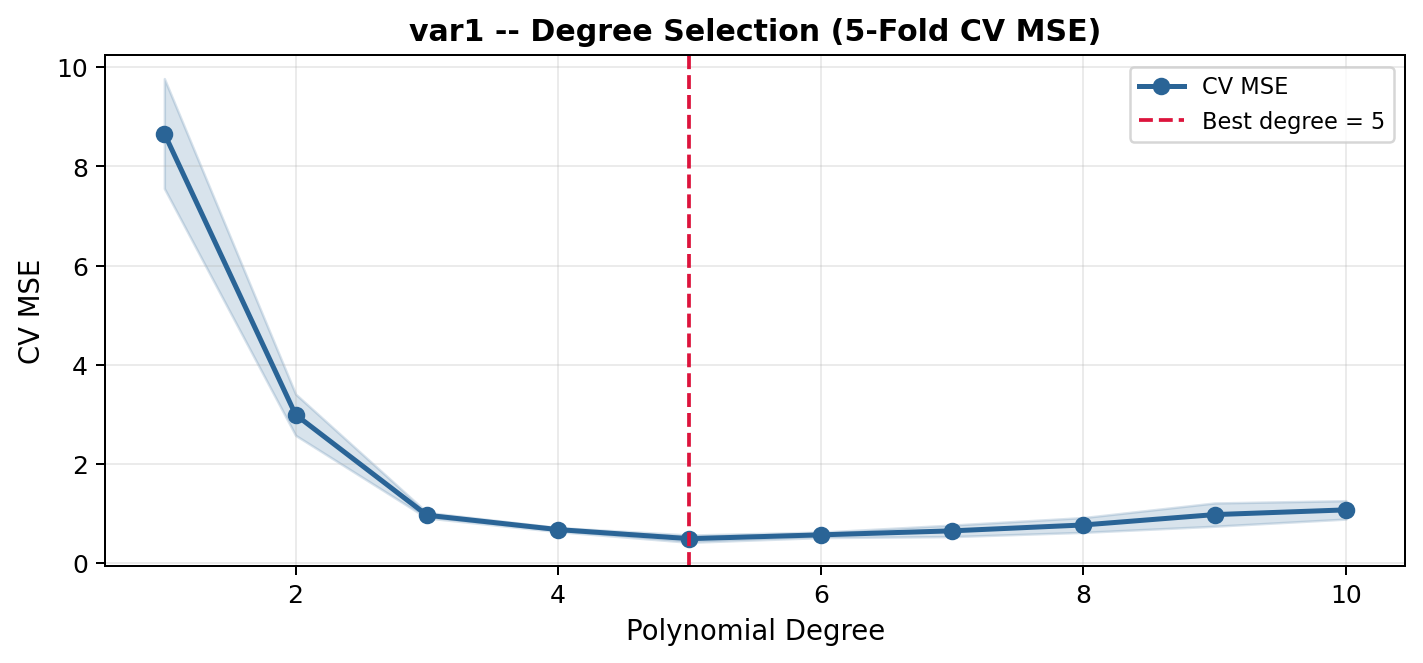
\includegraphics[
        width=0.88\textwidth,
        height=0.25\textheight,
        keepaspectratio
    ]{figures/var1_degree_vs_error.png}
    \caption{5-fold cross-validation MSE for polynomial degrees 1--10
    on the \texttt{var1} dataset.  The dashed red line marks the
    selected degree.}
    \label{fig:var1-degree}
\end{figure}

The cross-validation MSE decreases sharply from degree 1 to degree 5
and then levels off or increases slightly at higher degrees, indicating
overfitting.  \textbf{Degree 5} is selected as the optimal degree for
\texttt{var1}.

\subsection{Final Model}

The final \texttt{var1} model configuration is:

\begin{itemize}
    \item Polynomial degree: 5
    \item Regression method: Ridge (\texttt{RidgeCV})
    \item Regularization parameter $\alpha = 24.4205$: selected
    automatically by \texttt{RidgeCV} over a 50-point logarithmic
    grid in $[10^{-4}, 10^4]$
    \item Feature standardization: \texttt{StandardScaler}
    \item Total polynomial terms: 462
\end{itemize}

The final model is retrained on the complete training dataset (1000
samples).  Its training-set performance is:

\begin{table}[H]
\centering
\small
\begin{tabular}{lc}
\toprule
Metric & Value \\
\midrule
Training MSE & 0.20328 \\
Training $R^2$ & 0.97912 \\
\bottomrule
\end{tabular}
\caption{Training performance of the final \texttt{var1} model.}
\end{table}

These figures describe performance on the training data and should not
be interpreted as the hidden test-set evaluation.

For reference, the cross-validation results across all evaluated
degrees for \texttt{var1} are:

\begin{table}[H]
\centering
\small
\begin{tabular}{cc}
\toprule
Polynomial Degree & CV MSE \\
\midrule
1  & 8.66342 \\
2  & 2.99288 \\
3  & 0.96692 \\
4  & 0.67628 \\
5  & \textbf{0.49331} \\
6  & 0.57071 \\
7  & 0.65166 \\
8  & 0.76998 \\
9  & 0.97906 \\
10 & 1.07415 \\
\bottomrule
\end{tabular}
\caption{5-fold cross-validation MSE for all polynomial degrees
evaluated on \texttt{var1}.  The bold entry indicates the selected
degree.}
\end{table}

\subsection{Residual Analysis}

Figure~\ref{fig:var1-residuals} presents the residual analysis for the
final \texttt{var1} model.

\begin{figure}[H]
    \centering
    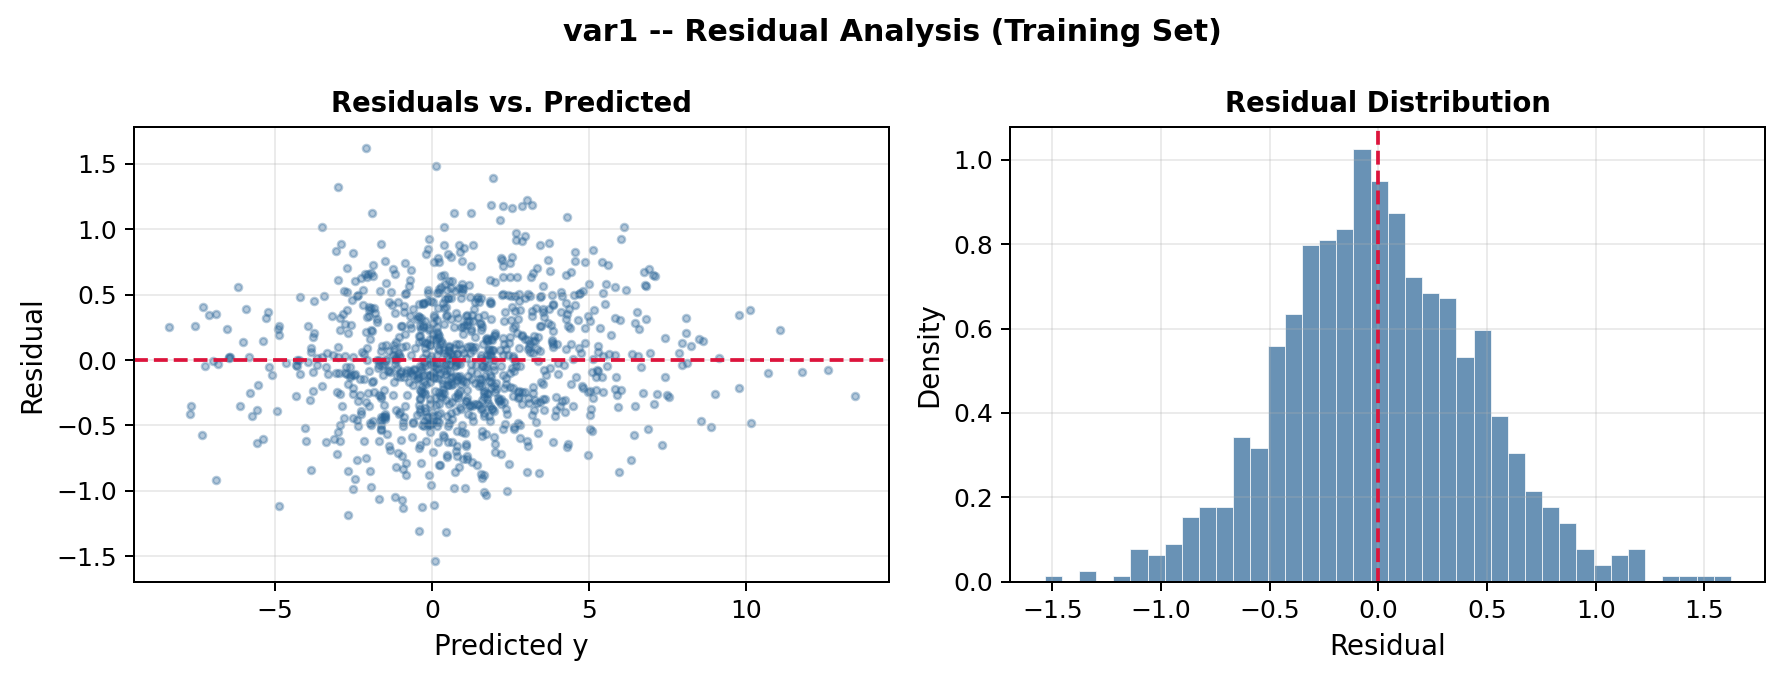
\includegraphics[
        width=0.88\textwidth,
        height=0.24\textheight,
        keepaspectratio
    ]{figures/var1_residuals.png}
    \caption{Residual analysis for the final \texttt{var1} model.
    \emph{Left}: residuals plotted against predicted values.
    \emph{Right}: distribution of residuals.}
    \label{fig:var1-residuals}
\end{figure}

The residuals are spread approximately symmetrically around zero with
no pronounced structure, which is consistent with a well-specified
model.

% ==================================================
\section{Problem 2: \texttt{var2}}
% ==================================================

\subsection{Dataset}

The \texttt{var2} dataset is associated with the problem of
\emph{Subterranean Thermal Reservoir Mapping}. It contains three input
variables,

\[
x_1,\; x_2,\; x_3,
\]

and the target variable $y$.  Both the training and test datasets
contain 1000 samples each.  The target variable is available only in
the training dataset.

The maximum permitted polynomial degree for this problem is 20.

\subsection{Degree Selection}

Polynomial degrees 1 through 20 were evaluated using 5-fold
cross-validation with the same Ridge pipeline used for \texttt{var1}.

Figure~\ref{fig:var2-degree} shows the mean validation MSE and the
corresponding $\pm1$ standard-deviation band.

\begin{figure}[H]
    \centering
    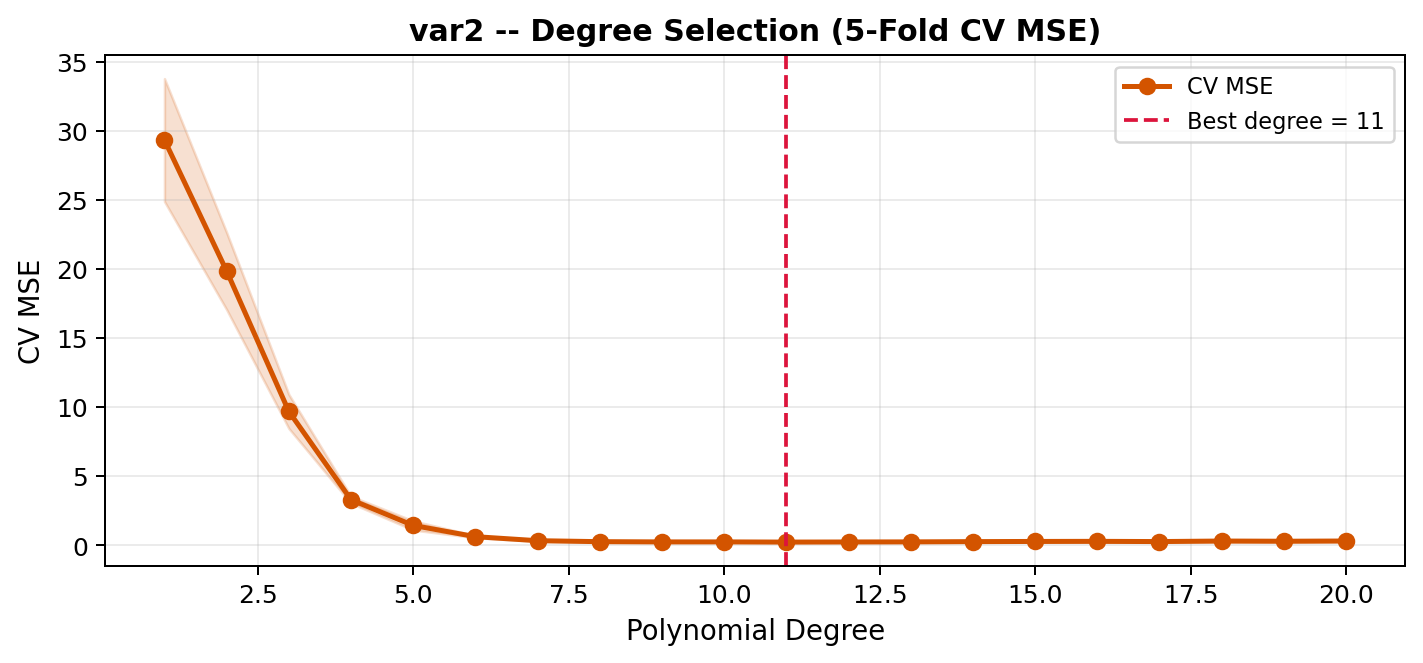
\includegraphics[
        width=0.88\textwidth,
        height=0.25\textheight,
        keepaspectratio
    ]{figures/var2_degree_vs_error.png}
    \caption{5-fold cross-validation MSE for polynomial degrees 1--20
    on the \texttt{var2} dataset.  The dashed red line marks the
    selected degree.}
    \label{fig:var2-degree}
\end{figure}

The validation MSE decreases rapidly for low degrees and then
stabilises, reaching a minimum at degree 11.  Higher degrees show
no further improvement.  The cross-validation results for a selection
of degrees are shown below.

\begin{table}[H]
\centering
\small
\begin{tabular}{ccc}
\toprule
Polynomial Degree & CV MSE & CV $R^2$ \\
\midrule
1  & 29.34065 & 0.26060 \\
2  & 19.85724 & 0.49514 \\
3  &  9.69979 & 0.75272 \\
4  &  3.30961 & 0.91375 \\
5  &  1.44844 & 0.96324 \\
6  &  0.63411 & 0.98391 \\
7  &  0.34300 & 0.99128 \\
8  &  0.27327 & 0.99297 \\
9  &  0.25543 & 0.99341 \\
10 &  0.25587 & 0.99343 \\
11 & \textbf{0.24284} & \textbf{0.99372} \\
12 &  0.25031 & 0.99355 \\
13 &  0.25714 & 0.99339 \\
14 &  0.27629 & 0.99295 \\
15 &  0.28879 & 0.99266 \\
16 &  0.29618 & 0.99250 \\
17 &  0.28042 & 0.99284 \\
18 &  0.31837 & 0.99198 \\
19 &  0.30358 & 0.99229 \\
20 &  0.32038 & 0.99189 \\
\bottomrule
\end{tabular}
\caption{5-fold cross-validation results for all polynomial degrees
evaluated on \texttt{var2}.  Degree 11 achieves the lowest CV MSE
and is selected for the final model.}
\end{table}

\textbf{Degree 11} achieves the lowest validation MSE (0.24284) among
all evaluated degrees and is therefore selected for the final
\texttt{var2} model.

\subsection{Final Model}

The final \texttt{var2} model configuration is:

\begin{itemize}
    \item Polynomial degree: 11
    \item Regression method: Ridge (\texttt{RidgeCV})
    \item Regularization parameter $\alpha = 1.2068$: selected
    automatically by \texttt{RidgeCV} over a 50-point logarithmic
    grid in $[10^{-4}, 10^4]$
    \item Feature standardization: \texttt{StandardScaler}
    \item Total polynomial terms: 364
\end{itemize}

The final model is retrained on the complete training dataset.  Its
training-set performance is:

\begin{table}[H]
\centering
\small
\begin{tabular}{lc}
\toprule
Metric & Value \\
\midrule
Training MSE & 0.16019 \\
Training $R^2$ & 0.99602 \\
\bottomrule
\end{tabular}
\caption{Training performance of the final \texttt{var2} model.}
\end{table}

\subsection{Residual Analysis}

Figure~\ref{fig:var2-residuals} shows the residual behavior of the
final degree-11 Ridge model on the training set.

\begin{figure}[H]
    \centering
    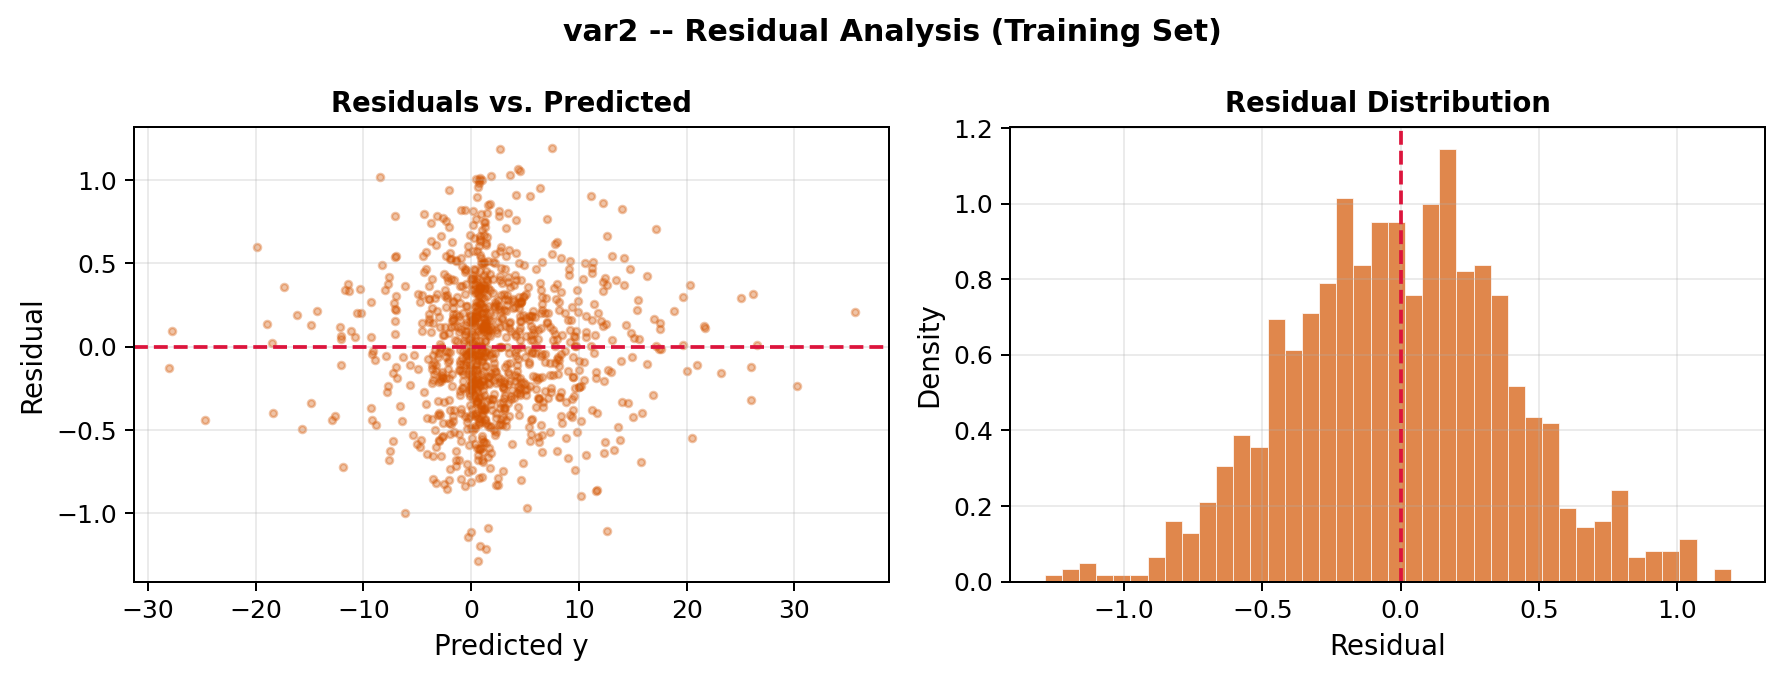
\includegraphics[
        width=0.88\textwidth,
        height=0.24\textheight,
        keepaspectratio
    ]{figures/var2_residuals.png}
    \caption{Residual analysis for the final \texttt{var2} model.
    \emph{Left}: residuals plotted against predicted values.
    \emph{Right}: distribution of residuals.}
    \label{fig:var2-residuals}
\end{figure}

The residuals are centered near zero with no evident pattern, and
their distribution is approximately symmetric, which is consistent
with a well-fitted model.

% ==================================================
\section{Inference and Prediction}
% ==================================================

After degree selection and final model training, the trained pipelines
are applied to the corresponding test datasets:

\[
X_{\mathrm{test}}
\longrightarrow
\text{Polynomial Feature Expansion}
\longrightarrow
\text{StandardScaler}
\longrightarrow
\text{Trained Ridge Model}
\longrightarrow
\hat{y}_{\mathrm{test}}.
\]

Because the true target values of the test datasets are withheld, the
test-set MSE and $R^2$ cannot be computed locally.

The final prediction files are:

\begin{itemize}
    \item \texttt{BT2024103\_pred\_var1.csv}
    \item \texttt{BT2024103\_pred\_var2.csv}
\end{itemize}

Each file contains a single column \texttt{y} with the predicted
values for the corresponding test dataset (1000 rows each).

% ==================================================
\section{Implementation}
% ==================================================

The entire solution is contained in a single script,
\texttt{ml\_assignment\_solution.py}, organized into the following
logical stages:

\begin{itemize}
    \item \textbf{Data loading}: reads the four CSV files
    (\texttt{train\_var1}, \texttt{test\_var1}, \texttt{train\_var2},
    \texttt{test\_var2}).
    \item \textbf{Degree selection} (\texttt{find\_best\_degree}):
    iterates over candidate degrees, builds the Ridge pipeline, and
    evaluates it with 5-fold CV using both MSE and $R^2$ scoring.
    \item \textbf{Final model training} (\texttt{train\_final\_model}):
    refits the pipeline on the full training set using a fine
    logarithmic grid of $\alpha$ values via \texttt{RidgeCV}.
    \item \textbf{Prediction \& saving}: applies each trained pipeline
    to the corresponding test features and saves the results as CSV.
    \item \textbf{Visualization}: generates the degree-selection and
    residual-analysis figures used in this report.
\end{itemize}

All computations use \texttt{scikit-learn} pipelines to ensure that
feature scaling is estimated only on the training fold during
cross-validation, preventing data leakage.

% ==================================================
\section{Conclusion}
% ==================================================

Polynomial regression was applied to both personalized datasets using
a unified Ridge regularization pipeline and 5-fold cross-validation
for degree selection.

For \texttt{var1} (Power Plant Steam Turbine Optimization), polynomial
degree 5 was selected.  The final degree-5 Ridge model
($\alpha = 24.4205$) achieved a training MSE of 0.20328 and a training
$R^2$ of 0.97912, with 462 polynomial features.

For \texttt{var2} (Subterranean Thermal Reservoir Mapping), polynomial
degree 11 was selected based on the lowest validation MSE
(CV MSE = 0.24284, CV $R^2$ = 0.99372) across degrees 1--20.
The final degree-11 Ridge model ($\alpha = 1.2068$) achieved a training
MSE of 0.16019 and a training $R^2$ of 0.99602, with 364 polynomial
features.

The trained models were applied to the corresponding test datasets,
producing the two required prediction CSV files
(\texttt{BT2024103\_pred\_var1.csv} and
\texttt{BT2024103\_pred\_var2.csv}).

\end{document}
